\section{Boolean Autoencoders}
Boolean autoencoders correspond to the case where $\mathbb{F} = \mathbb{G} = \{0, 1\}$, $A$ and $B$ are classes of Boolean functions, and $\Delta$ is the Hamming distance. Traditionally, a Boolean function is defined as a mapping from $\{0, 1\}^n$ to $\{0, 1\}$. but here we use the same term more generally to refer to Boolean vector functions, that is functions from $\{0, 1\}^n$ to $\{0, 1\}^m$ which of course can be seen as $m$ Boolean functions. 
\[
    \mathbb{H}^p \ni \begin{bmatrix}
        0\\
        1\\
        \vdots\\
        1\\
        0
    \end{bmatrix}   \to 
    \begin{bmatrix}
        1\\
        0\\
        0\\
        \vdots\\
        1\\
        0\\
        1
    \end{bmatrix} \in \mathbb{H}^m
\]

In the general framework, the sets $\mathcal{A}, \mathcal{B}$ contain all possible Boolean functions of the right dimensions. Given $k$ binary column vectors $p_1, \dots, p_k$ in the $n$-dimensional hypercube $\mathbb{H}^n$, we define the corresponding binary majority vector Majority($p$) in $\mathbb{H}^n$ by taking in each row $j$ the majority of the corresponding components $p_{ij}$. When $n$ is even, there can be ties in which case one can flip a fair coin to assign the corresponding value. 
\vspace{1.5cm}
\[
    k\text{-rows }
  \begin{bmatrix}
    \flag{left}{1} & 0  & 1 & 1 & 1 & \flag{right}{0}\\
    1 & 1 & 0 & 1 & 0  & 1 \\
    0 & 0 & 1 & 0 & 1  & 0\\
    1 & 1 & 0 & 1 & 1  & 0 \\
  \end{bmatrix}
  \hspace{3cm}
  \highlight{N}
  \flag{left}{1}
    \flag{right}{} 
  \highlight{NT}
\]
\overlay{
  \draw[->, thick, red, dashed] (N) -- (NT)
    node [pos=0.48, above] {$p_1$};
  \node[above of = N ] { $n$-element rows   };
  \node[below of = NT] { $Majority(p_1)$ };
}

\begin{lemma}
    The vector \text{Majority}(p) is a vector in $\mathbb{H}^n$ closest to the center of gravity of the vectors $p_1, \dots, p_k$ and it minimizes the function $E(q) = \sum_{i=1}^k \Delta(p_i, q)$.
\end{lemma}
\begin{proof}
    The center of gravity is the vector $c$ in $\mathbb{R}^n$ with coordinates 
    \[
        c_j = \dfrac{\left(\sum\limits_{i=1}^{k} p_{ji}\right)}{k}
    \]
    So, each $c_j$ is the average of the $j$-th components of the vectors $p_1, \dots, p_k$.
    For any $j$, $(p)_j$ is the closest binary value to $c_j$. Furthermore:
    \[
        \sum_{i=1}^k \Delta(\text{Majority}(p), p_i) = \sum_{i=1}^k \sum_{j=1}^n \Delta(\text{Majority}(p)_j,p_{ij}) =   \sum_{j=1}^n \left(\sum_{i=1}^k \Delta(\text{Majority}(p)_j,p_{ij})\right)
    \]
    and each term in the last sum is minimized by the majority vector. 
\end{proof}

A \textbf{Voronoi partition} of $\mathbb{H}^n$ generated by the vectors $p_1, \dots, p_k$ is a partition of $\mathbb{H}^n$ into $k$ regions $\mathcal{C}^{Vor}(p_1), \dots, \mathcal{C}^{Vor}(p_k)$ such that for each $x$ in $\mathbb{H}^n$:
\[
    x \in \mathcal{C}^{Vor}(p_i) \iff \Delta(x, p_i) \leq \Delta(x, p_j) \text{ for all } j \neq i    
\]
\newpage
And this can be visualized as: 
    \begin{multicols}{2}
        \begin{center}
            \begin{figure}[H]
                \centering
                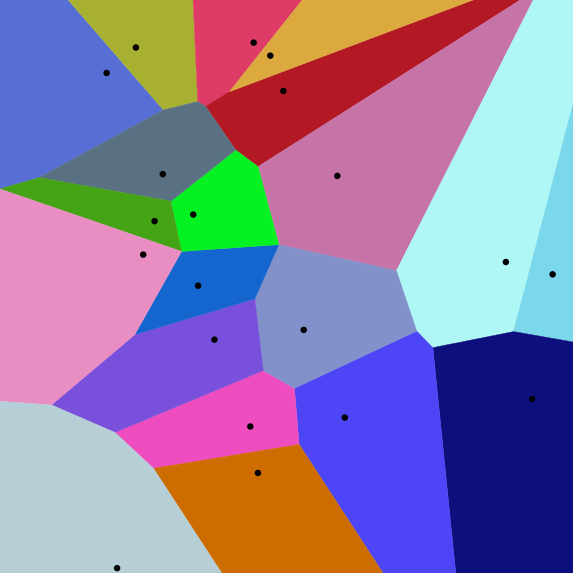
\includegraphics[width=0.3\textwidth]{./Images/Euclidean_Voronoi_diagram.png}
                \caption{Voronoi diagram with Euclidean distance metric}
            \end{figure}
        \end{center}
        \begin{center}
            \begin{figure}[H]
                \centering
                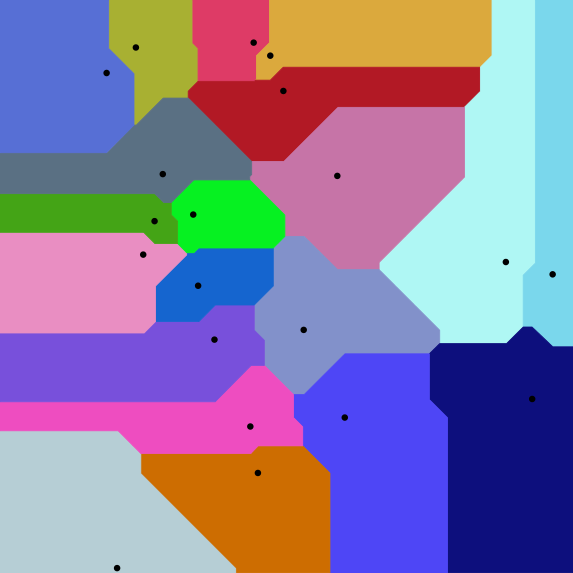
\includegraphics[width=0.3\textwidth]{./Images/Manhattan_Voronoi_Diagram.png}
                \caption{Voronoi diagram with Manhattan distance metric}
            \end{figure}
        \end{center}
    \end{multicols}

Recall that autoencoders performs a mapping of the input space $\mathbb{H}^n$ into a lower-dimensional space $\mathbb{H}^p$ and then back to the original space. The mapping is done by two functions $A$ and $B$ that are learned from the data. The mapping is done in two steps:
\[
    x \xrightarrow{B} h \xrightarrow{A} y
\]

\begin{theorem}
    \textbf{Fixed layer solution}: if the $A$ mapping is fixed , then the optimal mapping $B^*$ is given by $B^*(x) = h_i$ for any $x$ in $\mathcal{C}_i = \mathcal{C}^{Vor}(A(h_i))$. Conversely, if $B$ is fixed, then the optimal mapping $A^*$ is given by $A^*(h_i) = \text{Majority}\left[\mathcal{X} \cap B^{-1}(h_i)\right]$ 
\end{theorem}
\begin{proof}
    Assume first that $A$ is fixed . Then for each of the $2^p$ possible Boolean vectors $h_1, \dots, h_{2^{p}}$ of the hidden layer, $A(h_1), \dots, A(h_{2^p})$ provide $2^p$ points (centroids) in the hypercube $\mathbb{H}^n$. One can build the corresponding Voronoi partition by assigning each point of $\mathbb{H}^n$ to its closest centroid, breaking ties arbitrarily, thus forming a partition of $\mathbb{H}^n$ into $2^p$ corresponding clusters $\mathcal{C}_1, \dots, \mathcal{C}_{2^p}$, with $\mathcal{C}_i = \mathcal{C}^{Vor}(A(h_i))$. The optimal mapping $B^*$ is then given by $B^*(x) = h_i$ for any $x$ in $\mathcal{C}_i$.

    If we consider the input-output layers to have a cardinality of 4 and the hidden layer to have a cardinality of 2, then this would mean that there would be $2^2 = 4$ centroids given by the $A$ mapping in the space $\mathbb{H}^4$ showed in figure:

        \begin{figure}[H]
            \centering
            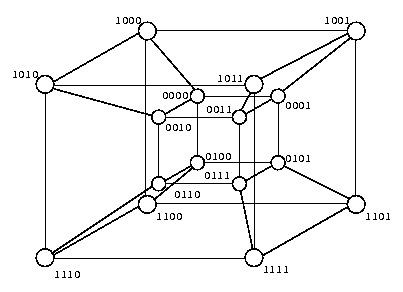
\includegraphics[width=0.5\textwidth]{./Images/Hypercube4Dimensions.png}
            \caption{Hypercube in 4 dimensions}
        \end{figure}
    So, the Voronoi partition would be the partition of the hypercube into 4 regions using as metric the Hamming distance, i.e. the number of edges that need to be crossed to go from one point to each centroid.\\

    Conversely, assume that $B$ is fixed. Then for each of the $2^p$ possible Boolean vectors $h_1, \dots, h_{2^{p}}$ of the hidden layer, let $B^{-1}(h_i) = \{x \in \mathbb{H}^n : B(x) = h_i\}$. To minimize the reconstruction error, $A^*$ must map $h_i$ onto a point $y$ of $\mathbb{H}^n$ minimizing the sum of Hamming distances to points in $\mathcal{X} \cap B^{-1}(h_i)$. By Lemma 3.1 the minimum is realized by the component-wise majority vector $A^*(h_i) = \text{Majority}[\mathcal{X} \cap B^{-1}(h_i)]$, breaking ties arbitrarily. Note that this solution minimizes the distortion on the training set. The generalization or total distortion however, is minimized by $A^*(h_i) = \text{Majority}[B^{-1}(h_i)]$. In some situations, one may have the additional constraint that the output vector must belong to the training. With this additional constraint the optimal solution is $A^*(h_i)$ should be the vector $\mathcal{X}$ that is closest to the vector $\text{Majority}[\mathcal{X} \cap B^{-1}(h_i)]$. 
\end{proof}
